% Synchronized to r35302

\marklabel{sec:OPTSAMBAPOINTANDPRINT:XP}{\section{SAMBA\_LPD - Configuration de Point'n'Print sous Windows XP}}

Cette section décrit la configuration et l'utilisation d'un client sur Windows XP
avec Point'n'Print.

Tout d'abord, le serveur d'impression doit être "trouvé". Pour cela vous pouvez
utiliser par exemple l'environnement réseau (Figure~\ref{fig:sambalpd:icon-networking-environment}
ou \ref{fig:sambalpd:networking-environment:4}). Dans l'exemple qui suit, le
groupe de travail est "GARDEN" et le serveur fli4l "ODIN". Le pilote d'imprimante
que vous souhaitez installer, est une Brother HL-2240D.

\begin{figure}[hbt!]
\centering
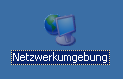
\includegraphics[]{image001}
\caption{Environnement réseau~: icône sur le bureau}
\label{fig:sambalpd:icon-networking-environment}
\end{figure}

\begin{figure}[hbt!]
\centering
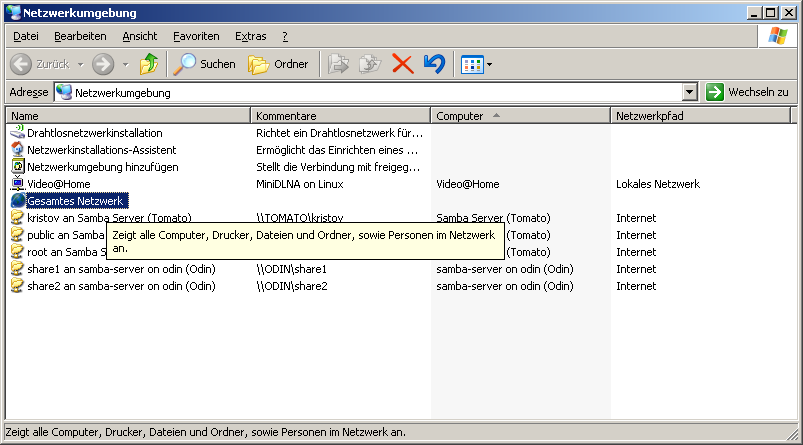
\includegraphics[width=\columnwidth]{image002}
\caption{Environnement réseau~: vue générale}
\label{fig:sambalpd:networking-environment:1}
\end{figure}

\begin{figure}[hbt!]
\centering
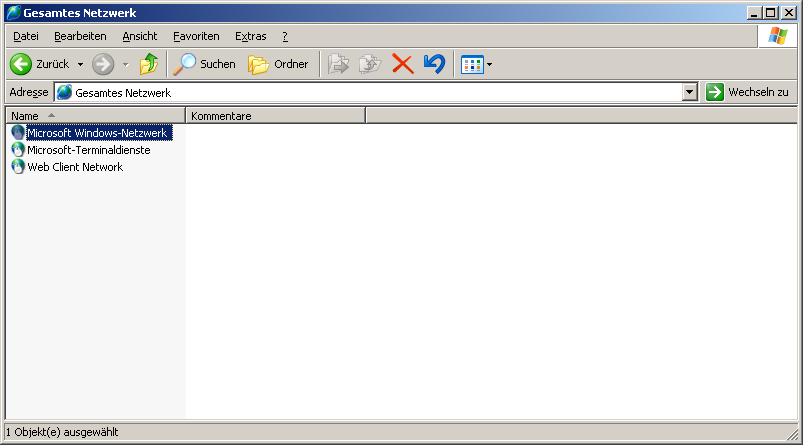
\includegraphics[width=\columnwidth]{image003}
\caption{Environnement réseau~: sélectionnez le type de réseau}
\label{fig:sambalpd:networking-environment:2}
\end{figure}

\begin{figure}[hbt!]
\centering
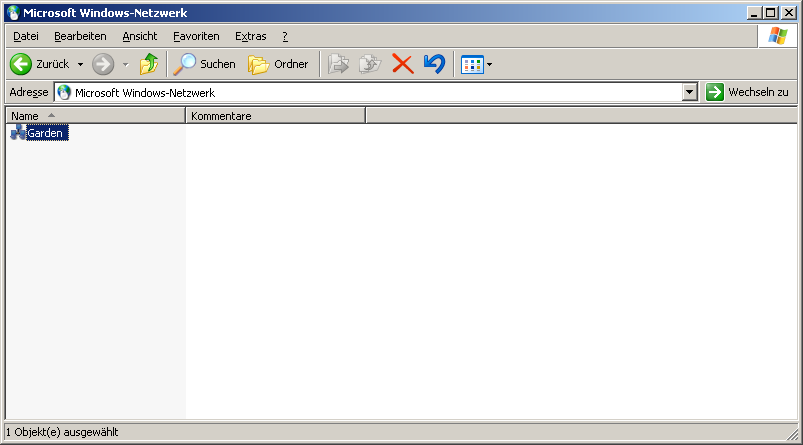
\includegraphics[width=\columnwidth]{image004}
\caption{Environnement réseau~: sélectionnez le groupe de travail}
\label{fig:sambalpd:networking-environment:3}
\end{figure}

\begin{figure}[hbt!]
\centering
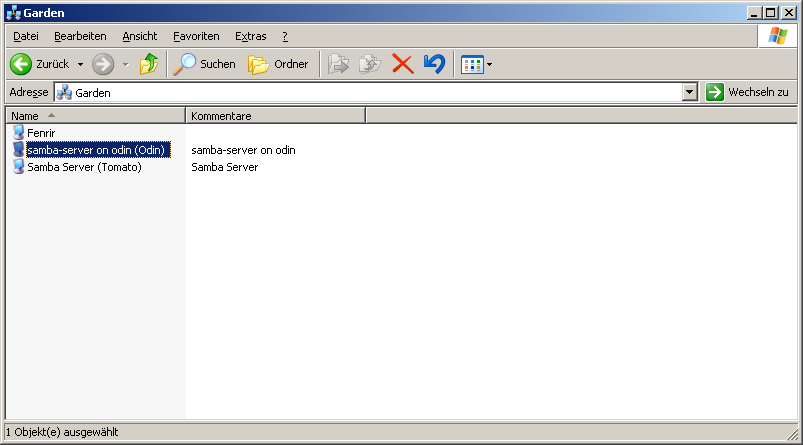
\includegraphics[width=\columnwidth]{image005}
\caption{Environnement réseau~: sélectionnez le serveur d'impression fli4l}
\label{fig:sambalpd:networking-environment:4}
\end{figure}

Si vous avez trouvé le serveur d'impression fli4l, vous pouvez ouvrir en double-cliquant
sur la fenêtre qui affiche les services (Abb.~\ref{fig:sambalpd:services}).
Ensuite vous sélectionnez "Imprimantes et télécopieurs". Vous devez voir
la liste de toutes les imprimantes configurées sur le serveur d'impression fli4l.
Maintenant, vous sélectionnez l'imprimante souhaitée, dans le menu contextuel
vous sélectionnez "Propriétés" (Abb.~\ref{fig:sambalpd:printerproperties}).
Vous allez avoir un message (Abb.~\ref{fig:sambalpd:no-driver:1}) qui indique
qu'il n'y a pas de pilote installé pour cette imprimante (ce qui est vrai).
Vous devez confirmer "Non" à ce message, car nous allons installer le pilote
via une méthode différente.

\begin{figure}[hbt!]
\centering
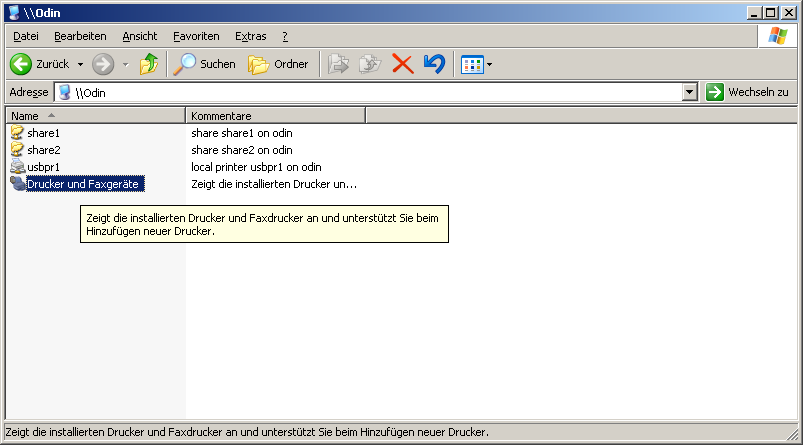
\includegraphics[width=\columnwidth]{image006}
\caption{Services du serveur}
\label{fig:sambalpd:services}
\end{figure}

\begin{figure}[hbt!]
\centering
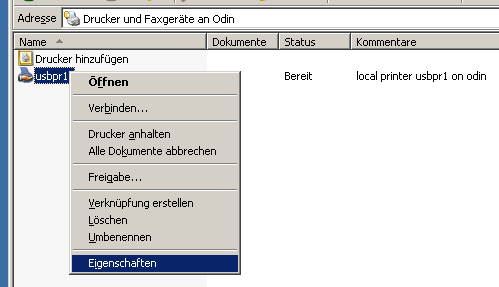
\includegraphics[width=\columnwidth]{image007}
\caption{Sélectionnez Propriétés de l'imprimante}
\label{fig:sambalpd:printerproperties}
\end{figure}

\begin{figure}[hbt!]
\centering
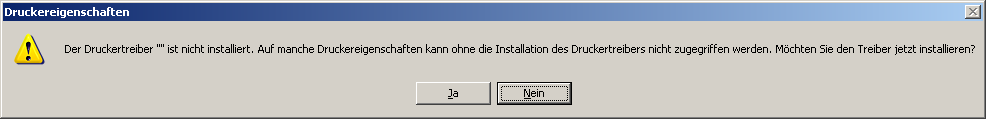
\includegraphics[width=\columnwidth]{image008}
\caption{Le pilote de l'imprimante est manquant (1)}
\label{fig:sambalpd:no-driver:1}
\end{figure}

Cela va ouvrir la boîte de dialogue Propriétés. Vous sélectionnez l'onglet
"Avancé" puis vous cliquez sur le bouton "Nouveau pilote"
(Abb.~\ref{fig:sambalpd:props-start-setup}). Cela conduit au début de
"l'assistant installation de l'imprimante" (Abb.~\ref{fig:sambalpd:setup-start}).
Avec "Suivant" vous sélectionnez le pilote (Abb.~\ref{fig:sambalpd:setup-choose-driver:1}).
Si le pilote souhaité n'est pas trouvé, vous pouvez spécifer le "support
de média" pour trouver le chemin vers le répertoire du pilote (il peut
être par exemple situé sur le CD d'installation de l'imprimante); Dans ce cas,
une deuxième liste de pilotes sera disponibles, à partir de laquelle vous
devez sélectionner le pilote (Abb.~\ref{fig:sambalpd:setup-choose-driver:2}).
Après la confirmation avec le bouton "Suivant", vous obtenez un message de 
l'assistant qui a terminé l'installation avec succès (Abb.~\ref{fig:sambalpd:setup-end}).
Mais se n'est pas vrai, parce que après avoir sélectionné le bouton "Terminer",
le pilote est copié depuis le serveur fli4l et ensuite activé
(Abb.~\ref{fig:sambalpd:driver-copy}).

\begin{figure}[hbt!]
\centering
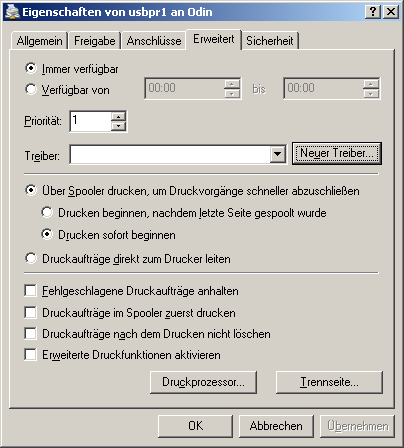
\includegraphics[width=0.8\columnwidth]{image009}
\caption{Propriétés de l'imprimante~: l'installation du pilote commence}
\label{fig:sambalpd:props-start-setup}
\end{figure}

\begin{figure}[hbt!]
\centering
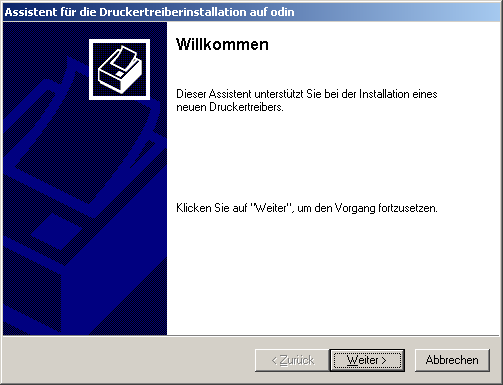
\includegraphics[width=\columnwidth]{image010}
\caption{Propriétés de l'imprimante}
\label{fig:sambalpd:setup-start}
\end{figure}

\begin{figure}[hbt!]
\centering
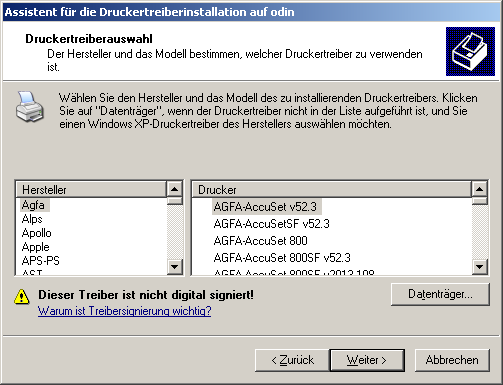
\includegraphics[width=0.7\columnwidth]{image011}
\caption{Installation du pilote~: sélection du pilote 1}
\label{fig:sambalpd:setup-choose-driver:1}
\end{figure}

\begin{figure}[hbt!]
\centering
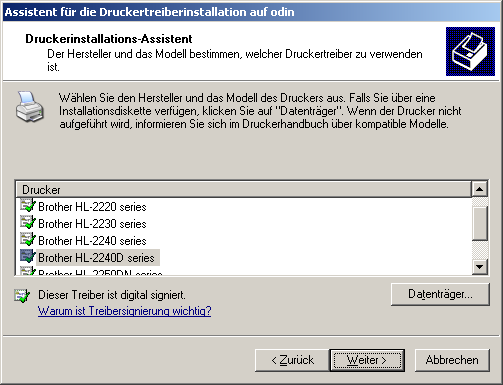
\includegraphics[width=0.7\columnwidth]{image012}
\caption{Installation du pilote~: sélection du pilote 2}
\label{fig:sambalpd:setup-choose-driver:2}
\end{figure}

\begin{figure}[hbt!]
\centering
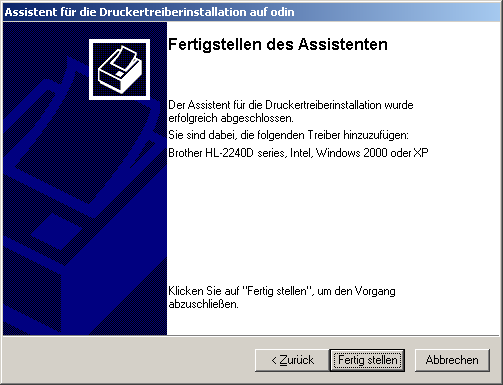
\includegraphics[width=\columnwidth]{image013}
\caption{Installation du pilote~: l'assistant a terminé}
\label{fig:sambalpd:setup-end}
\end{figure}

\begin{figure}[hbt!]
\centering
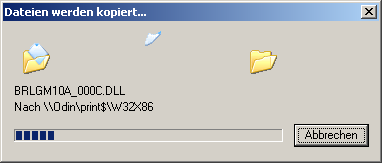
\includegraphics[width=\columnwidth]{image014}
\caption{Installation du pilote~: copie du pilote}
\label{fig:sambalpd:driver-copy}
\end{figure}

vous pouvez voir dans la boîte de dialogue Propriétés que le pilote
sélectionné est installé, il est affiché dans la fenêtre "Pilote"
(Abb.~\ref{fig:sambalpd:setup-completed}). Maintenant vous devez sortir
de la boîte de dialogue Propriétés en cliquant sur "OK". Là encore,
vous obtenez un message indiquant que le pilote est manquant
(Abb.~\ref{fig:sambalpd:no-driver:2}), cette fois quelle absurdité,
car le pilote est bien installé. Donc sélectionnée à nouveau "Non",
il est possible aussi installer nouveau un pilote. Maintenant, vous pouvez
revenir sur "Imprimantes et télécopieurs", et rebaptiser le nom de
l'imprimante pour Windows en fonction du pilote choisi.
(Abb.~\ref{fig:sambalpd:installed}). Cela ne pose pas de problème,
l'accès au serveur d'impression fli4l est toujours possible.

\begin{figure}[hbt!]
\centering
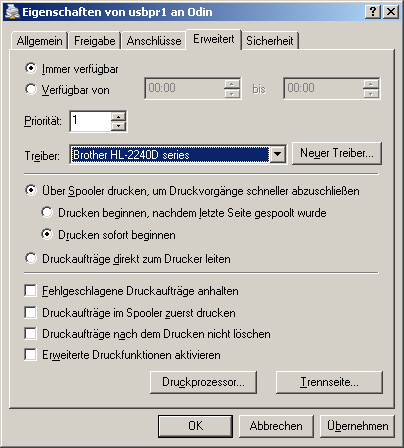
\includegraphics[width=\columnwidth]{image015}
\caption{Installation complète du pilote}
\label{fig:sambalpd:setup-completed}
\end{figure}

\begin{figure}[hbt!]
\centering
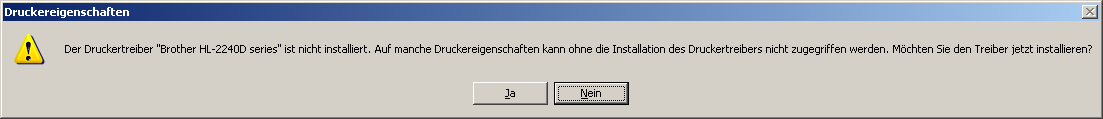
\includegraphics[width=\columnwidth]{image016}
\caption{Le pilote d'imprimante est manquant (2)}
\label{fig:sambalpd:no-driver:2}
\end{figure}

\begin{figure}[hbt!]
\centering
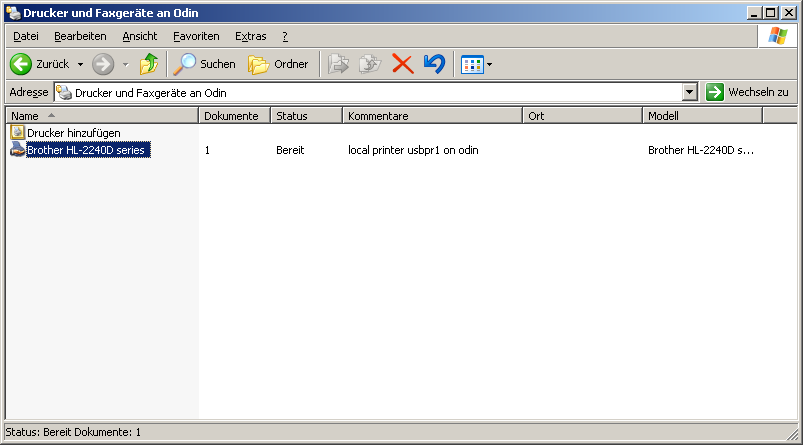
\includegraphics[width=0.8\columnwidth]{image017}
\caption{La partie 1 de l'installation de l'imprimante est achevée}
\label{fig:sambalpd:installed}
\end{figure}

Nous n'avons pas encore fini, nous devons paramètrer l'imprimante par défaut.
Pour ce faire, retournez dans la boîte de dialogue de l'imprimante
(Abb.~\ref{fig:sambalpd:printerproperties}) et dans l'onglet "Avancé" cliquez sur
le bouton "Impression pas défaut" (Abb.~\ref{fig:sambalpd:props-reloaded:1}). (Ce bouton
n'est pas visible avant la configuration et donc nous ne pouvions pas y accéder plutôt).
Maintenant ouvrez la fenêtre de dialogue du pilote (Abb.~\ref{fig:sambalpd:props-reloaded:2}).
Dans cette boîte de dialogue les paramètres de l'imprimante souhaités doivent être
maintenant réglés. Habituellement, vous devez configurer le papier "ordinaire" et
le format "A4". Si tous les paramètres sont correctes, néanmoins vous pouvez modifier
un paramètre avec un retour arrière~- cela est nécessaire pour que Windows enregistre
vraiment les paramètres sur le serveur fli4l, vous pouvez quitter la boîte de dialogue
et cliquer sur "OK".

\begin{figure}[hbt!]
\centering
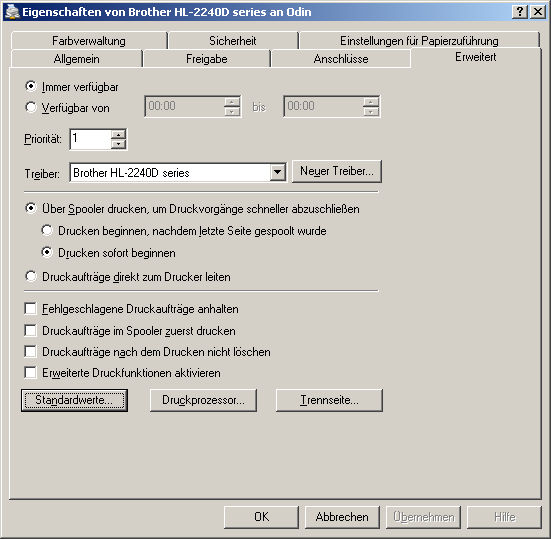
\includegraphics[width=0.8\columnwidth]{image018}
\caption{Définissez les valeurs par défaut (1)}
\label{fig:sambalpd:props-reloaded:1}
\end{figure}

\begin{figure}[hbt!]
\centering
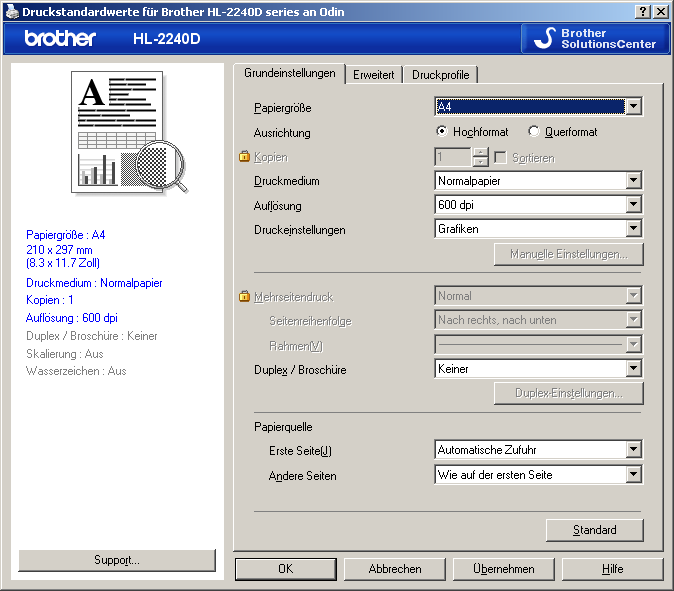
\includegraphics[width=\columnwidth]{image019}
\caption{Définissez les valeurs par défaut (2)}
\label{fig:sambalpd:props-reloaded:2}
\end{figure}

Maintenant, nous sommes arrivés~! La configuration côté serveur est terminée. Si vous
voulez utiliser l'imprimante que vous venez de configurer, vous devez vous connecter
sur celle-ci (Abb.~\ref{fig:sambalpd:connect:1}). Un message d'avertissement apparaît
sur les dangers du pilote installé (Abb.~\ref{fig:sambalpd:connect:2}) vous devez
confirmer. Enfin l'imprimante connectée apparaît dans l'environnement réseau
(Abb.~\ref{fig:sambalpd:printer-environment}). C'est parti~!

\begin{figure}[hbt!]
\centering
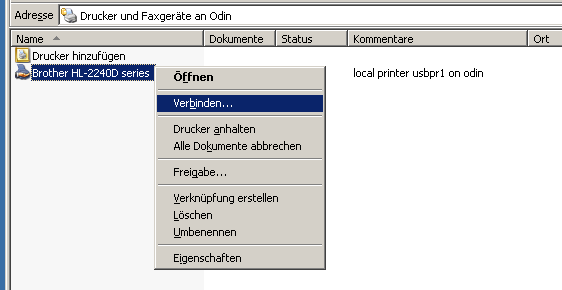
\includegraphics[width=\columnwidth]{image020}
\caption{Connexion à l'imprimante (1)}
\label{fig:sambalpd:connect:1}
\end{figure}

\begin{figure}[hbt!]
\centering
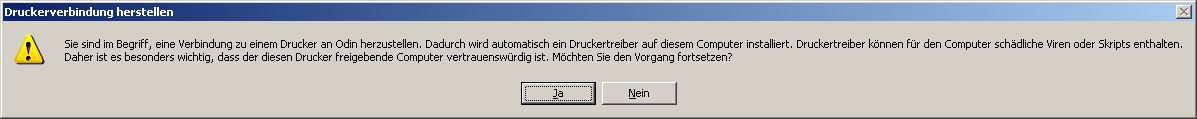
\includegraphics[width=\columnwidth]{image021}
\caption{Connecter à l'imprimante (2)}
\label{fig:sambalpd:connect:2}
\end{figure}

\begin{figure}[hbt!]
\centering
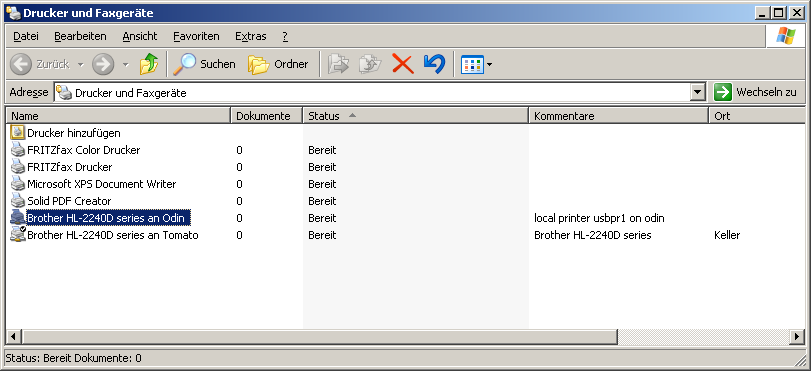
\includegraphics[width=\columnwidth]{image022}
\caption{L'imprimante est connectée dans l'environnement réseau}
\label{fig:sambalpd:printer-environment}
\end{figure}
